
\chapter{Theory}
\section{Modeling of cameras}

Since all cameras project a 3D scene onto a 2D plane, there will be information lost about the depth of the image. It is therefore not possible to calculate the exact placement of an object from a single picture, unless you have extra information about the objects in the picture. For this reason it is easy to create a projection in a 3D scene, but hard to create a scene from a projection. In addition to this, the amount of pixels and the field of view also affect the information and detail in the captured image. The most basic camera model is called the pinhole model, and is applicable for most cameras without high distortion lenses.

\subsection{pinhole projection} \label{sec:pinhole}
The pinhole model is based on the first camera, the Camera Obscura, made in 1568. It captures a scene by projecting straight light rays through a common focal point, and through a plane. The projection itself is made from where the light rays intersect the projection plane. The focal length, $f$, and the image plane size will then decide the field of view, $\theta_x$ and $\theta_y$, as shown in Figure~\ref{fig:pinhole}. 

\begin{figure}[!htb]
    \centering

    \tdplotsetmaincoords{80}{145}
    \begin{tikzpicture}[tdplot_main_coords, scale = 1.8]
    
        \tdplotsetrotatedcoords{0}{-90}{90}
        \draw[tdplot_rotated_coords, ->] (-0.7,0,0) -- (2,0,0) node[below right]{$X$};
        \draw[tdplot_rotated_coords, ->] (0,-0.5,0) -- (0,1,0) node[right]{$Y$};
        \draw[tdplot_rotated_coords, dashed] (0,0,-0.5) -- (0,0,9.2);
        \draw[tdplot_rotated_coords, ->] (0,0,9.2) -- (0,0,10) node[below]{$z,Z$};
        
        \pgfmathsetmacro{\rvec}{8}
        \pgfmathsetmacro{\imgradius}{3}
        \pgfmathsetmacro{\thetavec}{12}
        \pgfmathsetmacro{\phivec}{8}
        
        \coordinate (O) at (0,0,0);
        \tdplotsetcoord{P1}{\rvec}{90 -\phivec}{180 - \thetavec}
        \tdplotsetcoord{longP1}{\rvec*1.1}{90 -\phivec}{180 - \thetavec}
        \tdplotsetcoord{P2}{\rvec}{90 +\phivec}{180 - \thetavec}
        \tdplotsetcoord{longP2}{\rvec*1.1}{90 +\phivec}{180 - \thetavec}
        \tdplotsetcoord{P3}{\rvec}{90 + \phivec}{180 + \thetavec}
        \tdplotsetcoord{longP3}{\rvec*1.1}{90 +\phivec}{180 + \thetavec}
        \tdplotsetcoord{P4}{\rvec}{90 - \phivec}{180 + \thetavec}
        \tdplotsetcoord{longP4}{\rvec*1.1}{90 -\phivec}{180 + \thetavec}
        
        \tdplotsetcoord{IMG1}{\imgradius}{90 -\phivec}{180 - \thetavec}
        \tdplotsetcoord{IMG2}{\imgradius}{90 +\phivec}{180 - \thetavec}
        \tdplotsetcoord{IMG3}{\imgradius}{90 +\phivec}{180 + \thetavec}
        \tdplotsetcoord{IMG4}{\imgradius}{90 -\phivec}{180 + \thetavec}
        \coordinate (IMGC) at (-2.906,0,0);
        
        \shade[tdplot_rotated_coords, ball color=blue!50, opacity = 0.7] (0,0,8) circle (1cm); 

        \tdplotsetrotatedcoordsorigin{(IMGC)} %\imgradius*sin(90-\phivec)*cos(180-\thetavec)
        \shade[tdplot_rotated_coords, ball color=blue!50, opacity = 0.7] (0,0,0) circle (0.375);
        \draw[tdplot_rotated_coords, ->] (-0.7,0,0) -- (2,0,0) node[below right]{$x$};
        \draw[tdplot_rotated_coords, ->] (0,-0.5,0) -- (0,1,0) node[right]{$y$};
        
        \draw[] (IMG1) -- (IMG2) -- (IMG3) -- (IMG4) -- cycle;
      
        \draw[] (0,0,0.75) -- (0,0,0.85); \draw[] (0,0,0.8) -- (-2.906,0,0.8); \draw[] (-2.906,0,0.75) -- (-2.906,0,0.85);
        \draw[] (-1.45,0,1) node{$f$};
        
        \draw[thick, opacity = 0.3] (O) -- (P1); \draw[dashed, opacity = 0.3] (P1) -- (longP1);
        \draw[thick, opacity = 0.3] (O) -- (P2); \draw[dashed, opacity = 0.3] (P2) -- (longP2);
        \draw[thick, opacity = 0.3] (O) -- (P3); \draw[dashed, opacity = 0.3] (P3) -- (longP3);
        \draw[thick, opacity = 0.3] (O) -- (P4); \draw[dashed, opacity = 0.3] (P4) -- (longP4);
        
        \tdplotsetthetaplanecoords{180-\thetavec}
        \tdplotdrawarc[tdplot_rotated_coords]{(O)}{5}{90-\phivec}{90+\phivec}{anchor=west}{$\theta_y$}
        \tdplotsetrotatedcoords{0}{\phivec}{90}
        \tdplotdrawarc[tdplot_rotated_coords]{(O)}{5}{90-\thetavec}{90+\thetavec}{anchor=south}{$\theta_x$}
        
        
    \end{tikzpicture}

    \caption{Pinhole projection with the image plane between the focal point and the object}
    \label{fig:pinhole}
    
\end{figure}

Using the properties of similar triangles, the relationship between the World coordinates, $X,Y,Z$ and the image coordinates $x,y$ becomes:

\begin{align}
    tan(\phi_x) &= \frac{x}{f} = \frac{X}{Z} & tan(\phi_y) &= \frac{y}{f} = \frac{Y}{Z} \label{eq:pinhole_tan_relation} \\
    x &= f\frac{X}{Z} & y &=f\frac{Y}{Z}
    \label{eq:pinhole_relation}
\end{align}

As seen in Equation \eqref{eq:pinhole_relation}, the relationship between the sizes nonlinear. In order to present this in matrix form, the homogenous coordinates $p=[x,y,1]^\top$ and $P=[X,Y,Z,1]^\top$ are used. The matrix transformation is shown in Equation~\eqref{eq:pinhole_matrix}, with the imtermediate step $p^*$ being $p$ scaled by $Z$.

\begin{align}
    p^* &= \begin{bmatrix}
        x^* \\ y^* \\ z^*
    \end{bmatrix} = \begin{bmatrix}
        f & 0 & 0 & 0 \\
        0 & f & 0 & 0 \\
        0 & 0 & 1 & 0
    \end{bmatrix}\begin{bmatrix}
        X \\ Y \\ Z \\ 1
    \end{bmatrix} &
    p &= \frac{1}{z^*}p^*
    \label{eq:pinhole_matrix}
\end{align}

Since the light rays need to pass through the pinhole and onto the image plane, it is not possible to have a field of view larger than $180^\circ$. As seen in Equation~\eqref{eq:pinhole_matrix}, the projected object is also scaled by the distance to it, causing the points where the vertical field of view is $180^\circ$ to be singular. 

In a digital camera, the image plane consists of a small chip with a discrete amount of light sensitive elements, or pixels. Defining a new pixel coordinate frame to consist of the image pixels, with the origin in the upper left corner, as shown in Figure~\ref{fig:rel_img_pixel}. Using $W$ and $H$ as the image width and height in pixels, the transformation from image coordinates to pixel coordinates will be as shown in Equation~\eqref{eq:pixel_transform}.

\begin{figure}[!htb]
    \centering
    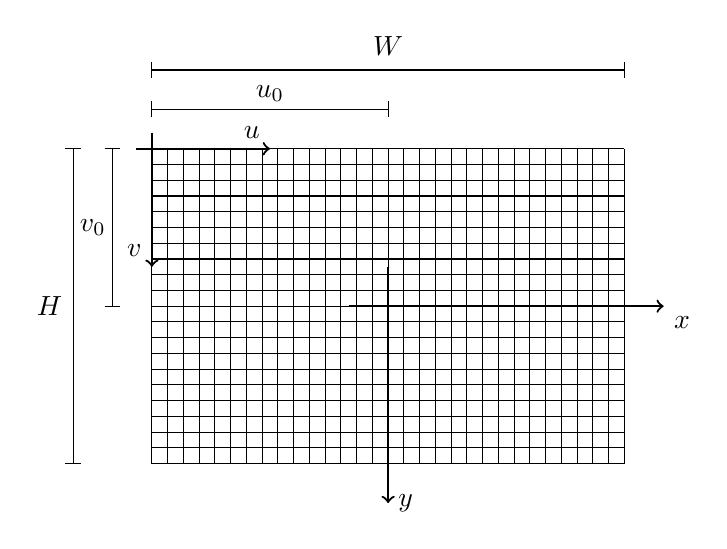
\begin{tikzpicture}[scale = 1.0]
    
    \draw[thick, ->] (-0.5,0,0) -- (3.5,0,0) node[below right]{$x$};
    \draw[thick, ->] (0,0.5,0) -- (0,-2.5,0) node[right]{$y$};
    \draw[thick, ->] (-3.2,2,0) -- (-1.5,2,0) node[above left]{$u$};
    \draw[thick, ->] (-3,2.2,0) -- (-3,0.5,0) node[above left]{$v$};
    
    \draw[] (-3,3,0) -- (3,3,0); \draw[] (-3,2.9,0) -- (-3,3.1,0); \draw[] (3,2.9,0) -- (3,3.1,0);
    \draw[] (-3,2.5,0) -- (0,2.5,0); \draw[] (-3,2.4,0) -- (-3,2.6,0); \draw[] (0,2.4,0) -- (0,2.6,0);
    \draw[] (-1.5,2.7,0) node{$u_0$};
    \draw[] (0,3.3,0) node{$W$};
    
    \draw[] (-4,2,0) -- (-4,-2,0); \draw[] (-4.1,2,0) -- (-3.9,2,0); \draw[] (-4.1,-2,0) -- (-3.9,-2,0);
    \draw[] (-3.5,2,0) -- (-3.5,0,0); \draw[] (-3.6,2,0) -- (-3.4,2,0); \draw[] (-3.6,0,0) -- (-3.4,0,0);
    \draw[] (-3.75,1,0) node{$v_0$};
    \draw[] (-4.3,0,0) node{$H$};
    
    \foreach \yline in {-2,-1.8,...,2} {
        \draw[] (-3, \yline, 0) -- (3, \yline, 0);
    } %end foreach
    
    \foreach \xline in {-3,-2.8,...,3} {
        \draw[] (\xline, -2, 0) -- (\xline, 2, 0);
    } %end foreach
    
    \end{tikzpicture}
    
    \caption{Relationship between pixel and image coordinates}
    \label{fig:rel_img_pixel}
\end{figure}

\begin{equation}
    p^i = \begin{bmatrix}
        u \\ v \\ 1
    \end{bmatrix} = \begin{bmatrix}
        \frac{W}{2x_{max}} & 0 & u_0 \\
        0 & \frac{H}{2y_{max}} & v_0 \\
        0 & 0 & 1
    \end{bmatrix}p =
    \begin{bmatrix}
        \frac{W}{2x_{max}} & 0 & u_0 \\
        0 & \frac{H}{2y_{max}} & v_0 \\
        0 & 0 & 1
    \end{bmatrix}\begin{bmatrix}
        x \\ y \\ 1
    \end{bmatrix}
    \label{eq:pixel_transform}
\end{equation}

\section{Distortions and wide angle pictures}

Wide angle image capture usually refers to pictures taken with a field of view grater than $60^\circ$. Increasing the field of view lets the camera capture more of the scene. However, the details also have to be compressed in order to fit in the image. This creates a trade-off between the amount of the scene captured and the level of detail. Increasing the resolution will reduce the amount of detail lost, but doing so also increases the amount of computation time needed to process the images.

As described in Section~\ref{sec:pinhole}, pinhole cameras are not able to capture elements that are straight to the side or behind the camera. This singularity can also be seen in Figure~\ref{fig:wide_angle_pinhole_nolens}, where the image plane would need to be infinitely big to capture elements at 90 degrees from the center image. In order to reliably capture wide angle pictures, wide angle cameras take advantage of lens distortion. Figure~\ref{fig:wide_angle_pinhole_lens} shows how a lens may be utilized to capture a wide angle picture onto a smaller image plane. The downside of this method is that elements towards the edges of the picture become compressed, causing straight lines to appear curved in the image. This type of distortion is called barrel distortion. Lenses that create barrel distortion in all radial directions from the image center is called a fisheye lens, are used in many wide angle cameras.

\begin{figure}[!htb]
    \centering
    \begin{subfigure}[b]{0.45\textwidth}
    \centering
    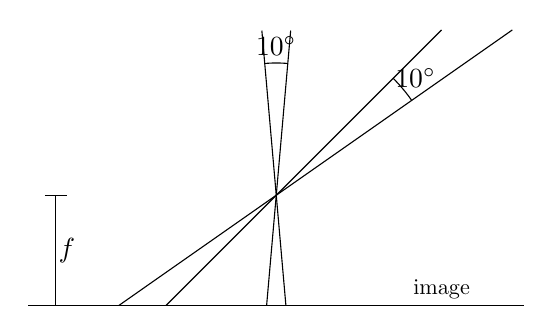
\begin{tikzpicture}[scale=0.7]
        \pgfmathsetmacro{\rvecimg}{2}
        \pgfmathsetmacro{\rvecscene}{3}
        
        \draw[] (0,0,0) -- (95:\rvecscene); \draw[] (0,0,0) -- (85:\rvecscene); 
        \draw[] (0,0,0) -- (-95:\rvecimg); \draw[] (0,0,0) -- (-85:\rvecimg);
        \draw[] (95:0.8*\rvecscene) arc (95:85:0.8*\rvecscene); \draw[] (90:0.9*\rvecscene) node{$10^\circ$};
        
        \draw[] (0,0,0) -- (45:1.414*\rvecscene); \draw[] (0,0,0) -- (35:1.743*\rvecscene); 
        \draw[] (0,0,0) -- (-135:1.414*\rvecimg); \draw[] (0,0,0) -- (-145:1.743*\rvecimg);
        \draw[] (45:\rvecscene) arc (45:35:\rvecscene); \draw[] (40:1.1*\rvecscene) node{$10^\circ$};
        
        \draw[] (-4.5,-\rvecimg,0) -- (4.5,-\rvecimg,0);
        \draw[] (3,-\rvecimg + 0.3,0) node[scale=0.8]{image};
        
        \draw[] (-4,-\rvecimg,0) -- (-4,0,0);
        \draw[] (-4.2,0,0) -- (-3.8,0,0);
        \draw[] (-3.8, -0.5*\rvecimg,0) node{$f$};
        
    \end{tikzpicture}
    \caption{Without lens distortion}
    \label{fig:wide_angle_pinhole_nolens}
    \end{subfigure}
    \begin{subfigure}[b]{0.45\textwidth}
    \centering
    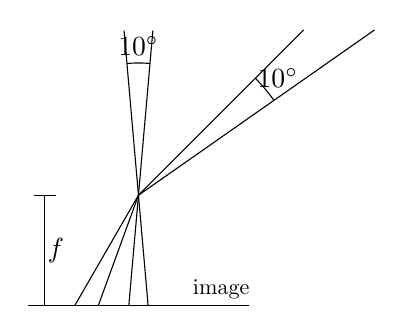
\begin{tikzpicture}[scale=0.7]
        \pgfmathsetmacro{\rvecimg}{2}
        \pgfmathsetmacro{\rvecscene}{3}
        
        \draw[] (0,0,0) -- (95:\rvecscene); \draw[] (0,0,0) -- (85:\rvecscene); 
        \draw[] (0,0,0) -- (-95:\rvecimg); \draw[] (0,0,0) -- (-85:\rvecimg);
        \draw[] (95:0.8*\rvecscene) arc (95:85:0.8*\rvecscene); \draw[] (90:0.9*\rvecscene) node{$10^\circ$};
        
        \draw[] (0,0,0) -- (45:1.414*\rvecscene); \draw[] (0,0,0) -- (35:1.743*\rvecscene); 
        \draw[] (0,0,0) -- (-110:1.064*\rvecimg); \draw[] (0,0,0) -- (-120:1.155*\rvecimg);
        \draw[] (45:\rvecscene) arc (45:35:\rvecscene); \draw[] (40:1.1*\rvecscene) node{$10^\circ$};
        
        \draw[] (-2,-\rvecimg,0) -- (2,-\rvecimg,0);
        \draw[] (1.5,-\rvecimg + 0.3,0) node[scale=0.8]{image};
        
        \draw[] (-1.7,-\rvecimg,0) -- (-1.7,0,0);
        \draw[] (-1.9,0,0) -- (-1.5,0,0);
        \draw[] (-1.5, -0.5*\rvecimg,0) node{$f$};
        
    \end{tikzpicture}
    \caption{With lens distortion}
    \label{fig:wide_angle_pinhole_lens}
    \end{subfigure}
    
    \caption{Amount of image space for different parts of the scene, using a pinhole camera, with and without a camera lens}
    \label{fig:wide_angle_pinhole}
    
\end{figure}

\subsection{Fisheye projection}

The lens distortion of a fisheye lens can be visualized and modeled through projecting the scene onto a sphere, and then project that sphere onto an image plane. Spherical coordiantes makes it is easier to describe points in the image plane, as the radial distances on the image plane is directly coupled to the angle a feature makes with the z-axis. Figure~\ref{fig:fisheye_spherical_projection} visualizes the projection, there the red lines represent a constant angle $\phi$.

Using the relationship betwen sperical and cartesian coordinates, $X = Rsin(\phi)cos(\theta)$, $Y = Rsin(\phi)sin(\theta)$ and $Z = Rcos(\phi)$, the polar coordinates $[R,\theta,\phi]^\top$ become:

\begin{equation}
    \begin{aligned}
        R = X^2 &+ Y^2 + Z^2 \\
        \theta = arctan\left(\frac{Y}{X}\right)\quad  ,& \quad \phi = arctan\left(\frac{\sqrt{X^2 + Y^2}}{Z}\right)
    \end{aligned}
    \label{eq:theory_polar_coords}
\end{equation}

\begin{figure}[!htb]
    \centering
    \tdplotsetmaincoords{70}{160}
    \begin{tikzpicture}[tdplot_main_coords, scale = 1.4]
    
    \coordinate (O) at (0,0,0);
    \tdplotsetrotatedcoords{0}{-90}{90}
    \draw[tdplot_rotated_coords, ->] (-0.5,0,0) -- (6,0,0) node[below right]{$X$};
    \draw[tdplot_rotated_coords, ->] (0,-0.5,0) -- (0,2.5,0) node[right]{$Y$};
    \draw[tdplot_rotated_coords, dashed] (0,0,-2.5) -- (0,0,6);
    \draw[tdplot_rotated_coords, ->] (0,0,6) -- (0,0,8) node[below]{$z,Z$};
    
    \tdplotsetcoord{P}{6}{65}{150}
    \draw[] (P) node[above right]{P}; \node at (P){\textbullet};
    \draw[] (O) -- (P);
    
    \tdplotsetcoord{ROTORIG}{7}{90}{180}
    \tdplotsetrotatedcoordsorigin{(ROTORIG)}
    \draw[tdplot_rotated_coords, ->] (180:0.3) arc (180:360:0.3);
    \draw[tdplot_rotated_coords] (0,-0.5,0) node{$\theta$};
    
    \tdplotsetcoord{IMGC}{2}{90}{0}
    \tdplotsetrotatedcoordsorigin{(IMGC)}
    \foreach \x in {-2,-1.5,...,2} {
        \draw[tdplot_rotated_coords] (\x,-2) -- (\x,2);
    }
    \foreach \y in {-2,-1.5,...,2} {
        \draw[tdplot_rotated_coords] (-2,\y) -- (2,\y);
    }
    \foreach \phi in {10,20,...,80} {
        \draw[tdplot_rotated_coords, color=red, opacity = 0.8] (0,0) circle({\phi/45});
    }
    \draw[tdplot_rotated_coords, thick, opacity = 0.8] (0,0) circle(2);
    
    \draw[tdplot_rotated_coords, ->] (-0.5,0,0) -- (4,0,0) node[below right]{$x$};
    \draw[tdplot_rotated_coords, ->] (0,-0.5,0) -- (0,2.5,0) node[right]{$y$};
    \draw[tdplot_rotated_coords, ->] (-2.5,-2,0) -- (2,-2,0) node[below right]{$u$};
    \draw[tdplot_rotated_coords, ->] (-2,-2.2,0) -- (-2,2,0) node[below]{$v$};
    
    \draw[tdplot_rotated_coords] (0,-2.3,0) -- (0,-2.3,2);
    \draw[tdplot_rotated_coords] (0,-2.2,0) -- (0,-2.4,0); \draw[tdplot_rotated_coords] (0,-2.2,2) -- (0,-2.4,2);
    \draw[tdplot_rotated_coords] (0,-2.5,1) node{$f$};
    
    \tdplotsetrotatedcoordsorigin{(O)}
    \draw[thick, tdplot_rotated_coords] (0:2) arc (0:360:2); 
    \foreach \angle in {-90,-95,...,-270} {
        \tdplotsetrotatedcoords{90}{\angle}{0}
        \draw[tdplot_rotated_coords, opacity = 0.7] (0:2) arc (0:180:2);
        
    }
    
    \foreach \angle in {10,20,...,80} {
        \coordinate (TMP) at ({-2*cos(\angle)},0,0);
        \tdplotsetrotatedcoordsorigin{(TMP)}
        \draw[tdplot_rotated_coords, color = red] (0:{2*sin(\angle)}) arc (0:360:{2*sin(\angle)});
    }
    
    \tdplotsetrotatedcoords{90}{-43}{0}
    \draw[tdplot_rotated_coords, ->] (90:5) arc (90:52:5);
    \draw[tdplot_rotated_coords] (70:5.3) node{$\phi$};
    
    \end{tikzpicture}
    
    \caption{Equiangular fisheye lens projection. Focal length exagerated for visual purposes.}
    \label{fig:fisheye_spherical_projection}
\end{figure}

In order to project the unit sphere onto a plane, there are different models. All of these describe different lens types, and by this gives the distortion model for a fisheye camera. Table~\ref{tab:theory_fisheye_lens_model} shows four different lens models used for fisheye cameras. the $r(\phi)$ represents the distance from the image center in the fisheye image plane. the relationship between the polar image coordinates $[r(\phi), \theta]^\top$ and the image coordinates $[x,y]^\top$ in Figure~\ref{fig:fisheye_spherical_projection}, can be seen in Equation~\eqref{eq:theory_equiangular_coords}. The mapping to pixel coordinates $[u,v]^\top$ is the same as described in Equation~\eqref{eq:pixel_transform}, where $x_max$ and $y_max$ is decided by $||r(\phi)||_2$.

\begin{align}
    r(\phi) &= f \cdot \phi & \theta &= \theta \nonumber \\
    x &= rcos(\theta) & y &= rsin(\theta)
    \label{eq:theory_equiangular_coords}
\end{align}

There are multiple different lens model for fisheye cameras. The Equiangular used in the above example is the simplest, and only incorporates radial distortion. In \cite{FisheyeCorke}, the models shown in Table~\ref{tab:theory_fisheye_lens_model} are presented. Another type of model is shown in Matlab's calibration guide for fisheye lens cameras\cite{MatlabFish}. This guide uses a model presented in \cite{FisheyeKalibration}, in addition to the ability to apply a stretch matrix and set distortion center. This model therefore provides much more customizability.

\begin{table}[!htb]
    \centering
    \begin{tabular}{|c|c|} \hline
        Lens model & radius $r(\phi)$ \\ \hline
        Equiangular & $k_1\phi$\\ \hline
        Stereographic & $k_1 tan\left(\frac{\phi}{2}\right)$\\ \hline
        Equisolid & $k_1 sin\left(\frac{\phi}{2}\right)$\\ \hline 
        Polynomial & $k_1 \phi + k_2 \phi^2 + ...$\\ \hline
    \end{tabular}
    \caption{Four different lens models for fisheye projection}
    \label{tab:theory_fisheye_lens_model}
\end{table}

\subsection{Cylindrical projection}

The goal of the cylindrical projection and camera types is to reduce the radial distortion and feature compression, while maintaining the ability to capture images with a horizontal field of view larger than $180^o$. Along the vertical y-axis, the cylindrical projection functions like a pinhole projection, where the mapping is identical to Equation~\eqref{eq:pinhole_relation}. For the horizontal axis, the polar coordinate $\theta$ is used, such that the mapping to the image plane becomes:

\begin{subequations}
\begin{equation}
    \theta = arctan\left(\frac{X}{Z}\right)
    \label{eq:cylindrical_theta}
\end{equation}
\begin{equation}
    y = R\frac{Y}{Z}
    \label{eq:cylindrical_y}
\end{equation}
\label{eq:cylindrical}
\end{subequations}

Theoretically this representation removes all vertical radial distortion, however it is still subject to the introduction of distortion through imperfect lenses or image plane alignment. Using the same vertical mapping as the pinhole model, also limits the vertical field of view, in the same manner as it would for the pinhole camera. Cameras using this projection types are not that common. This projection type is however highly suited to project and stitch pictures taken by a camera rotating around an axis, and is frequently used in panorama capture modes on digital cameras or mobile phones.

\subsection{Catadioptric projection}

Using internal mirrors to reflect the light, catadioptric lenses can achieve large focal lengths without increasing the physical length of the objective. This makes the technology ideal for telescopes and narrow angle imaging. The same principle has however been developed to include large field of view cameras and panoramic imaging, as seen in \cite{CatadioptricOmni}. 

\begin{figure}[!htb]
    \centering
    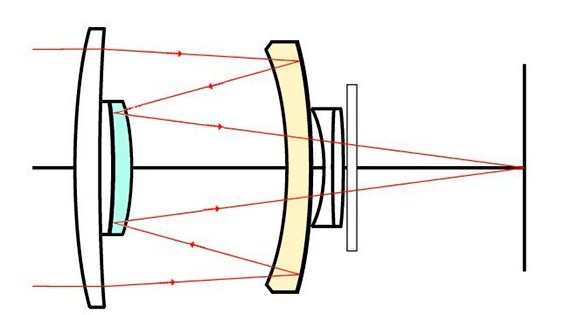
\includegraphics[width=0.6\textwidth]{rapport/fig/Theory/cata.jpeg}
    \caption{A simple catadiotric lens showing the central mirror, producing the blind spot. Downloaded from steemit.com/photography/@xenon2/catadioptric-lenses-old-is-new-again}
    \label{fig:theory_catadioptric_lens}
\end{figure}

Figure~\ref{fig:theory_catadioptric_lens} shows a simplified catadioptric mirror setup. Here we see that the mirror has to be placed within the field of view. This means that the catadioptric lens will always cause a blind spot. Shadows of the mirror mount may also appear in the image. To reduce this effect, the mount has to be made quite fragile. This makes the cameras unsuited for applications with significant vibrations.

The pixel mapping and field of view is highly dependent on the reflective surface used. Most surfaces will introduce similar radial distortions to the fisheye lens, but there has been developed catadioptric lenses, producing rectilinear projections \cite{RectilinearCatadioptric}, however this has to be mounted at a fixed distance from the ground, making them unfit for moving objects. Nayar S. K. made a wide angle, catadioptric lens \cite{CatadioptricOmni} with a single viewpoint, and proposes further a setup where two of these are mounted back to back to produce a full spherical image.

\subsection{Panomorph projection}

The panomorph lens types are designed around an non-uniform distribution of pixels within the field of view, and is patented by ImmerVision. This creates an opportunity to focus on important parts of the field of view, and enhance the resolution in these parts. This can couteract the problems wide angle cameras have with the reduces angular resolution, without increasing the image resolution. The non-uniform pixel distribution can also be tweaked to use more of the image sensors area \cite{PanomorphLowCostSurvailance}, and therefore utilizing more of the available resolution.

Different types of panomorphic lenses has been proposed for different applications. For example in 2010 it was proposed to use a panomorph lens in endoscopy\cite{endoscopypano}. This lens is based on the human eye, and its increased resolution around the center of vision. Other aplications include security cameras\cite{PanomorphEnhancesSurvailance}, where the outlying areas has been given increased resolution, to counteract the compact representation provided by normal fisheye cameras.

Since the pixel density varies within the field of view, the lens is more difficult to construct as well as model. As it closely resembles the fisheye lens, one could possibly achieve a quite good calibration using the polynomial model in \ref{tab:theory_fisheye_lens_model} or the unified model presented in \cite{FisheyeKalibration}. As they both support nonlinear radial distortion. The polynomial model would however need to be augmented with stretch parameters.

\section{Computer graphics}

Our eyes and cameras capture the 3D world from light hitting photosensitive elements. An object directly or partly behind another object will therefore be hidden in the picture, unless captured by a reflection. In addition to this, shadows, colors and lighting of objects in the scene are all based on how the light rays bounce around in the room, and eventually hit the camera lens. In computer graphics, there is no inherent concept of light. This means that all the effects that are based around light must be estimated or simulated. Since calculating light and shadow effects are quite expensive computationally, it is not uncommon to add shadow elements directly to the object texture, in order to optimize the for speed.

There are two main approaches: One approach is Ray tracing, which simulates light rays as they travel in straight lines from the camera center, through a pixel. When a ray hits an object, the ray is split in two, creating a shadow ray following the same trajectory through the object, and a reflection ray following the reflection trajectory. Ultimately these rays will find a light source, leave the scene. Usually the rays are limited to a number of bounces, to save some computation. This technique is incredibly powerful, and is used heavily in CGI effects for film making. However, the amount of computation necessary makes it hard to incorporate this in real-time applications.

The other approach is often referred to as rasterization, and is the one used most in real-time applications. Rasterization is a step in a larger pipeline of graphics computations, choosing which element to draw to which pixel. The main advantage Razterization has is it's short computation time and ability to be parallelized. As processing speed is very important in real time graphics production, and has also driven the graphics cards to be as effective as they are today. The downside of rasterization is that it looses a lot of information about the lighting in the scene, providing the shader much less information for the final coloring.

\subsection{Graphics projection}

Before the rasterization and the coloring(shading) of the pixels can be done, one must solve the visibility problems. This is one of the main difficulties in graphics programming. In simple terms, this consists of two tasks: \emph{Clipping}, which is the process of removing the parts that are outside the FoV, and \emph{Culling}, the process of deciding what is visible to the camera. While clipping of the FoV is straight forward, culling is not. The problem comes with transparency and reflections, where objects that are behind others, should still be visible or contribute to the final pixel color. 

In order to do these tasks effeciently, and to be able to use the same algorithms on different projection types, the scene is first projected into a normalized volume. This means that a projection in computer graphics is referencing a volume tranformation in $\mathbb{R}^3$, instead of a tranformation from $\mathbb{R}^3 \rightarrow \mathbb{R}^2$, which is referenced in the case of camera projections. The final transformation to an image plane happen in the rasterization and shading algorithm.

There are two main projection types used: orthographic and perspective. Orthographic projection is specially made to keep the scale of the object independent on how far away it is from the camera. This makes it ideal for schematics and other computer aided design, where the size of the drawing must be proportional to the real size of the object. The other type is perspective projection, and will be the one which is relevant for this project.

\subsection{Perspective projection}

The goal of perspective projection is to compress the scene into a normalized volume, while conserving the perspective properties. This means that object sizes are scaled with distance, the same way as in a pinhole camera. In Figure~\ref{fig:perspective_proj_yz}, a side view of this process is shown, in the yz-plane. The image shows two points $a$ and $b$, as well as their projected counterparts $a^*$ and $b^*$ in the normalized volume. $\Theta$ is in this case the vertical FoV.

\begin{figure}[!htb]
    \centering
        \begin{tikzpicture}[scale=1.0]
            \coordinate (O) at (0,0,0);
            \coordinate (OL) at (-7,0,0);
            \coordinate (OH) at (4,0,0);
        
            \draw[dashed, ->] (-7.3,0) -- (-1,0) node[below right]{$Z$};
            \draw[->] (-7,1.5) -- (-7,-1.5) node[above left]{$Y$};
            
            \draw[->] (1,0) -- (7.3,0) node[below right]{$z$};
            \draw[->] (4,3) -- (4,-3) node[right]{$y$};
            
            \tdplotsetrotatedcoordsorigin{(OH)}
            \draw[tdplot_rotated_coords] (-1.5,-1.5) -- (-1.5,1.5) node{\textbullet} node[below right]{$a^*$} -- (1.5,1.5) node{\textbullet} node[below right]{$b^*$}-- (1.5,-1.5) -- cycle;
            
            \draw[tdplot_rotated_coords] (1.5,0) node[below right]{\scriptsize $1$};
            \draw[tdplot_rotated_coords] (0,-1.5) node[below right]{\scriptsize $1$};
            \draw[tdplot_rotated_coords] (0,1.5) node[above right]{\scriptsize $-1$};
            \draw[tdplot_rotated_coords] (-1.5,0) node[below left]{\scriptsize $-1$};
        
            \tdplotsetrotatedcoordsorigin{(OL)}
            \draw[tdplot_rotated_coords, ->] (0,0) -- (15:5.5);
            \draw[tdplot_rotated_coords, ->] (0,0) -- (-15:5.5);
            
            \draw[tdplot_rotated_coords] (1.5, {1.5*tan(-15)}) -- (1.5,{1.5*tan(15)});
            \draw[tdplot_rotated_coords] (1.5, {1.5*tan(-15)}) -- (1.5,{1.5*tan(15)});
            
            \draw[tdplot_rotated_coords] (4, {4*tan(-15)}) -- (4,{4*tan(15)});
            \draw[tdplot_rotated_coords] (4, {4*tan(-15)}) -- (4,{4*tan(15)});
            
            \draw[tdplot_rotated_coords] (15:2) arc (15:-15:2);
            \draw[tdplot_rotated_coords] (2.2,0.2) node{$\Theta$};
            
            \draw[tdplot_rotated_coords] (1.5,{1.5*tan(15)}) node{\textbullet} node[above left]{$a$};
            \draw[tdplot_rotated_coords] (4,{4*tan(15)}) node{\textbullet} node[above left]{$b$};
            
            \draw[tdplot_rotated_coords] (0,-1.8) -- node[midway, above]{$d_n$} ++(1.5,0);
            \draw[tdplot_rotated_coords] (0,-1.9) -- (0,-1.7); \draw[tdplot_rotated_coords] (1.5,-1.9) -- (1.5,-1.7);
            \draw[tdplot_rotated_coords] (0,-2.2) -- node[midway, above]{$d_f$} ++(4,0);
            \draw[tdplot_rotated_coords] (0,-2.3) -- (0,-2.1); \draw[tdplot_rotated_coords] (4,-2.3) -- (4,-2.1);
            
        \end{tikzpicture}
    \caption{plane view of a perspective projection, with $a^*,b^*$ being the projected version of $a,b$}
    \label{fig:perspective_proj_yz}
\end{figure}

One important thing to note is the distances $d_n$ and $d_f$ these refer to the near and far clipping plane. These two parameter along with the FoV defines the volume which should be projected, and is shown in Figure~\ref{fig:theory_perspective_projection_volume}. As view distance greatly affects the amount of data that has to be processed, these parameters can be set in order to tell the renderer how near and how far to look. The roles of these parameters in the projection will be described later in this Section.

The relationship between the FoV and near clipping plane distance $d_n$ follows the same principle as for cameras, where $d_n$ can be seen as the focal length. This means that the FoV $\Theta$ is directly linked to $d_n$ and the size of the clipping plane. As seen in Figure~\ref{fig:perspective_proj_yz}, both point $a$ and $b$ are projected to $y=1$. Using the perspective relation of scale from Equation~\eqref{eq:pinhole_tan_relation}, and the scale parameter $s$, we find the relation between $y$ and $Y$, as shown in Equation~\eqref{eq:theory_perspective_y}. Here $a_y$ and $b_y$ are the y coordinates of $a$ and $b$.

\begin{equation}
    \begin{aligned}
        1 = y = s \frac{Y}{Z} = s \frac{a_y}{d_n} &= s \frac{b_y}{d_f} = s \cdot tan\left(\frac{\Theta}{2}\right) \quad ,for \quad \theta = \Theta \\\\
        \Rightarrow s &= \frac{1}{tan\left(\frac{\Theta}{2}\right)}
        \label{eq:theory_perspective_y}
    \end{aligned}
\end{equation}

To describe the projection of $X$ we may use the aspect ratio to form a relationship between the horizontal and vertical FoV. Equation \eqref{eq:theory_FOV_relationship} shows this, with the horizontal FoV denoted as $\Theta_H$. The projection of $X$ is shown in Equation~\eqref{eq:theory_perspective_x}.


\begin{equation}
    tan\left(\frac{\Theta_H}{2}\right) = \frac{W}{H}tan\left(\frac{\Theta}{2}\right) = \frac{1}{\rho}tan\left(\frac{\Theta}{2}\right) \quad , for \quad \rho = \frac{Height}{Width}
    \label{eq:theory_FOV_relationship}
\end{equation}
\begin{equation}
    x = \frac{1}{tan\left(\frac{\Theta_H}{2}\right)}\frac{X}{Z} = \frac{\rho}{tan\left(\frac{\Theta}{2}\right)}\frac{X}{Z}
    \label{eq:theory_perspective_x}
\end{equation}


\begin{figure}[!htb]
    \centering
    \tdplotsetmaincoords{80}{135}
    \begin{tikzpicture}[tdplot_main_coords, scale = 1.8]
    
        \tdplotsetrotatedcoords{0}{-90}{90}
        \draw[tdplot_rotated_coords, ->] (-0.7,0,0) -- (2,0,0) node[below right]{$X$};
        \draw[tdplot_rotated_coords, ->] (0,-0.5,0) -- (0,1,0) node[right]{$Y$};
        \draw[tdplot_rotated_coords, dashed] (0,0,-0.5) -- (0,0,9.2);
        \draw[tdplot_rotated_coords, ->] (0,0,9.2) -- (0,0,10) node[below]{$Z$};
        
        \pgfmathsetmacro{\rvec}{8}
        \pgfmathsetmacro{\imgradius}{2}
        \pgfmathsetmacro{\farplaneradius}{5}
        \pgfmathsetmacro{\thetavec}{12}
        \pgfmathsetmacro{\phivec}{8}
        
        \coordinate (O) at (0,0,0);
        \tdplotsetcoord{P1}{\rvec}{90 -\phivec}{180 - \thetavec}
        \tdplotsetcoord{longP1}{\rvec*1.1}{90 -\phivec}{180 - \thetavec}
        \tdplotsetcoord{P2}{\rvec}{90 +\phivec}{180 - \thetavec}
        \tdplotsetcoord{longP2}{\rvec*1.1}{90 +\phivec}{180 - \thetavec}
        \tdplotsetcoord{P3}{\rvec}{90 + \phivec}{180 + \thetavec}
        \tdplotsetcoord{longP3}{\rvec*1.1}{90 +\phivec}{180 + \thetavec}
        \tdplotsetcoord{P4}{\rvec}{90 - \phivec}{180 + \thetavec}
        \tdplotsetcoord{longP4}{\rvec*1.1}{90 -\phivec}{180 + \thetavec}
        
        \tdplotsetcoord{IMG1}{\imgradius}{90 -\phivec}{180 - \thetavec}
        \tdplotsetcoord{IMG2}{\imgradius}{90 +\phivec}{180 - \thetavec}
        \tdplotsetcoord{IMG3}{\imgradius}{90 +\phivec}{180 + \thetavec}
        \tdplotsetcoord{IMG4}{\imgradius}{90 -\phivec}{180 + \thetavec}
        
        \tdplotsetcoord{FAR1}{\farplaneradius}{90 -\phivec}{180 - \thetavec}
        \tdplotsetcoord{FAR2}{\farplaneradius}{90 +\phivec}{180 - \thetavec}
        \tdplotsetcoord{FAR3}{\farplaneradius}{90 +\phivec}{180 + \thetavec}
        \tdplotsetcoord{FAR4}{\farplaneradius}{90 -\phivec}{180 + \thetavec}
        \coordinate (IMGC) at ({-\imgradius*cos(16)},0,0);

        \tdplotsetrotatedcoordsorigin{(IMGC)} %\imgradius*sin(90-\phivec)*cos(180-\thetavec)
        
        \draw[draw=blue, fill=blue!30, opacity=0.3] (FAR1) -- (FAR2) -- (FAR3) -- (FAR4) -- cycle;
        \draw[draw=blue, fill=blue!30, opacity=0.3] (IMG3) -- (IMG4) -- (FAR4) -- (FAR3) -- cycle;
        \draw[draw=blue, fill=blue!30, opacity=0.3] (IMG3) -- (IMG2) -- (FAR2) -- (FAR3) -- cycle;
        \draw[draw=blue, fill=blue!30, opacity=0.3] (IMG1) -- (IMG2) -- (IMG3) -- (IMG4) -- cycle;
        \draw[draw=blue, fill=blue!30, opacity=0.3] (IMG1) -- (IMG2) -- (FAR2) -- (FAR1) -- cycle;
        \draw[draw=blue, fill=blue!30, opacity=0.3] (IMG4) -- (IMG1) -- (FAR1) -- (FAR4) -- cycle;
      
        \draw[] (0,0,0.75) -- (0,0,0.85); \draw[] (0,0,0.8) -- ({-2*cos(16)},0,0.8); \draw[] ({-2*cos(16)},0,0.75) -- ({-2*cos(16)},0,0.85);
        \draw[] (-1.45,0,1) node{$d_n$};
        \draw[] (0,0,1.25) -- (0,0,1.35); \draw[] (0,0,1.3) -- ({-5*cos(16)},0,1.3); \draw[] ({-5*cos(16)},0,1.25) -- ({-5*cos(16)},0,1.35);
        \draw[] (-2.5,0,1.5) node{$d_f$};
        
        \draw[thick, opacity = 0.3] (O) -- (P1); \draw[dashed, opacity = 0.3] (P1) -- (longP1);
        \draw[thick, opacity = 0.3] (O) -- (P2); \draw[dashed, opacity = 0.3] (P2) -- (longP2);
        \draw[thick, opacity = 0.3] (O) -- (P3); \draw[dashed, opacity = 0.3] (P3) -- (longP3);
        \draw[thick, opacity = 0.3] (O) -- (P4); \draw[dashed, opacity = 0.3] (P4) -- (longP4);
        
        \tdplotsetthetaplanecoords{180-\thetavec}
        \tdplotdrawarc[tdplot_rotated_coords]{(O)}{3}{90-\phivec}{90+\phivec}{anchor=west}{$\Theta$}
        \tdplotsetrotatedcoords{0}{\phivec}{90}
        \tdplotdrawarc[tdplot_rotated_coords]{(O)}{3}{90-\thetavec}{90+\thetavec}{anchor=south}{$\Theta_H$}
        
        
    \end{tikzpicture}
    \caption{Perspective projection Showing the projected scene volume}
    \label{fig:theory_perspective_projection_volume}
\end{figure}

In pinhole projection, the scaling caused by the distance $Z$ is implemented into the model through homogeneous coordinates. The same principle will be used for this projection. However, since the coordinate $z \in [-1,1]$ in the target volume, an additional parameter $w$ must be added. In order to provide the correct scale to the transformation, $w$ is set to equal $Z$. This can be seen on the bottom line of the projection matrix in Equation~\eqref{eq:perspective_projmat_temp}.

As there is no need for angular transformation when projecting $Z$ to $z$, $z$ will only depend on $Z$ and the scaling due to $w$. Knowing that the near clipping plane should be projected to $z=-1$, and the far clipping plane to $z=1$, we can make the system of equations shown in Equation~\eqref{eq:perspective_zeqs}. Here $K_{33}$ and $K_{34}$ refer to elements in the projection matrix $K$ in Equation~\eqref{eq:perspective_projmat_temp}. The pre-multiplication of $Z$ on the left and side of the equal sign is to incorporate the scaling of the homogeneous vector.

\begin{equation}
    \begin{aligned}
        zZ &= K_{33} Z + K_{34} &\\
        zd_n &= K_{33} d_n + K_{34} &, for \quad Z &= d_n \\
        zd_f &= K_{33} d_f + K_{34} &, for \quad Z &= d_f \\
        \Rightarrow K_{33} &= \frac{n+f}{n-f} & \quad \Rightarrow K_{34} &= \frac{2nf}{n-f}
    \end{aligned}
    \label{eq:perspective_zeqs}
\end{equation}


While the projection of $X$ and $Y$ more or less are equal for most renderer implementations, the projection of $Z$ is highly dependent on the chosen target cube, as well as the orientation of the Z-axis. Using the homogenous scene coordinates $P = [X,Y,Z,1]^\top$ and $p* = [x,y,z,w]^\top$ the transformation can be written as shown in Equation~\eqref{eq:perspective_projmat_temp}. Here $w = Z$ to scale $X$ and $Y$, and needs to be taken into account when calculating the $Z$ projection. Since both clipping planes have the z-axis as a plane normal in both the original scene, as well as the projected cube, $z$ will be independent on $X$ and $Y$ simplifying the computation to the set of two equations shown in Equation~\eqref{eq:perspective_zeqs}.


\begin{align}
    \begin{bmatrix}
        x \\ y \\ z \\ w
    \end{bmatrix} = KP = \begin{bmatrix}
        s & 0 & 0 & 0 \\
        0 & s & 0 & 0 \\
        0 & 0 & K_{33} & K_{34} \\
        0 & 0 & 1 & 0
    \end{bmatrix} \begin{bmatrix}
        X \\ Y \\ Z \\ 1
    \end{bmatrix} = \begin{bmatrix}
        \frac{\rho}{tan\left(\frac{\Theta}{2}\right)}& 0 & 0 & 0 \\
        0 & \frac{1}{tan\left(\frac{\Theta}{2}\right)}& 0 & 0 \\
        0 & 0 & \frac{d_n+d_f}{d_f-d_n} & \frac{2d_n d_f}{d_f-d_n} \\
        0 & 0 & 1 & 0
    \end{bmatrix} \begin{bmatrix}
        X \\ Y \\ Z \\ 1
    \end{bmatrix}
    \label{eq:perspective_projmat_temp}
\end{align}

In an ideal setting, there should be no need for a far clipping plane, meaning that all objects in the distance are drawn, no matter how far away they are. While this may differ from renderer to renderer, some implement funcionality for letting the the far clipping plane approach infinity. Equation~\eqref{eq:theory_inf_far_clip} how this can be implemented for the perspective projection, by letting $d_f \rightarrow \infty$. The final projection matrix is shown in Equation~\eqref{eq:theory_inf_proj_mat}.

\begin{equation}
    \begin{aligned}
    K_{33} = \lim_{d_f \rightarrow \infty} \frac{d_n+d_f}{d_f-d_n} =
    \lim_{d_f \rightarrow \infty} \frac{\frac{d_n}{d_f}+1}{1-\frac{d_n}{d_f}} = 
    \frac{1}{1} = 1 \\
    K_{34} = \lim_{f \rightarrow \infty} -\frac{2d_n d_f}{d_f-d_n} = 
    \lim_{d_f \rightarrow \infty} -\frac{2d_n}{1-\frac{d_n}{d_f}} =
    -\frac{2n}{1} = -2n
    \end{aligned}
    \label{eq:theory_inf_far_clip}
\end{equation}

\begin{equation}
    \begin{bmatrix}
        \frac{\rho}{arctan(\Theta/2)} & 0 & 0 & 0 \\
        0 & \frac{1}{arctan(\Theta/2)} & 0 & 0 \\
        0 & 0 & K_{33} & K_{34} \\
        0 & 0 & 1 & 0 
    \end{bmatrix} = \begin{bmatrix}
        \frac{1}{arctan(\theta/2)} & 0 & 0 & 0 \\
        0 & \frac{1}{arctan(\Theta/2)} & 0 & 0 \\
        0 & 0 & 1 & -2d_n \\
        0 & 0 & 1 & 0 
    \end{bmatrix}
    \label{eq:theory_inf_proj_mat}
\end{equation}


% \subsection{Ray Tracing}

% Ray tracing techniques have existed as a fully developed technique since 1986 \cite{raytraceblog}. Today, Ray tracing is highly used in film making for CGI, which is Computer-generated imagery to be applied on its own, or in the same frame as actual camera footage. The inherent ability ray tracing has to mimic real world light, enables the algorithms to produce very realistic images. The downside is that tracing light rays, all their reflections, refractions and shadows they cast, is really computationally expensive.

% Since 1986 much research has gone into improving the rendering time of these images. \cite{wald2009state} summarizes many of these, but also shows the conflicts between ray tracing approaches for video games, and approaches for movie making. The article states that the movie making approach is centered around making data structures for efficient computation, while more or less ignoring the building time of these structures. This can be backed up by Section 3 of \cite{carsmovie}, where the main focus is shown to be memory management and quality. In real time applications however, these data structures needs to be built and rebuilt, in addition to the computation, in real time. 

% Nvidia recently developed their RTX-series of graphics cards \cite{raytraceblog}, promising to revolutionize the ways shadows, reflections and lighting are shown in real-time image processing, with the use of ray tracing. Based on their launch event presentation \cite{NvidiaConference}, this will be realized by; the integration of ray tracing cores, a locally developed ray tracing acceleration algorithm and deep learning. The ray tracing cores are are specialized processing units, designed to parallelize ray tracing calculations, while the ray tracing acceleration refers to a search algorithm for finding intersections between light rays and objects. Lastly the deep learning portion uses a previously trained deep learning network, made specifically to upscale and fill in the gaps of lower quality images, with the goal of reducing the amount of rays needed to be calculated, as well as to perform anti-aliasing tasks.

\cleardoublepage